\documentclass[14pt]{extarticle}

\usepackage[T1]{fontenc}
\usepackage[utf8]{inputenc}

\usepackage[hidelinks]{hyperref}

\usepackage{microtype}

\usepackage{amssymb}
\usepackage{amsmath}
\usepackage{mathtools}
\usepackage{dsfont}

\usepackage{enumitem}

\usepackage{tikz}
\usetikzlibrary{cd, patterns, patterns.meta, decorations.pathmorphing}

\usepackage{geometry}
\geometry{a4paper, total={170mm, 252mm}, top=22mm}

\usepackage[skip=7pt]{parskip}

\usepackage{amsthm}
\usepackage{thmtools}

\declaretheoremstyle[
    headfont=\bfseries\color{green!80!black},
    bodyfont=\normalfont,
    notebraces={: }{},
    notefont=\color{green},
    headformat=\NAME$\;$\NUMBER\NOTE,
    postheadspace=\newline,
    mdframed={
        linewidth=2pt,
        rightline=false, topline=false, bottomline=false,
        linecolor=green, backgroundcolor=yellow!4,
        skipabove=3mm, skipbelow=3mm
    }
]{defbox}

\declaretheoremstyle[
    headfont=\bfseries\color{orange!80!black},
    bodyfont=\normalfont,
    notebraces={: }{},
    notefont=\color{orange},
    headformat=\NAME$\;$\NUMBER\NOTE,
    postheadspace=\newline,
    mdframed={
        linewidth=2pt,
        rightline=false, topline=false, bottomline=false,
        linecolor=orange, backgroundcolor=yellow!4,
        skipabove=3mm, skipbelow=3mm
    }
]{theorembox}

\declaretheoremstyle[
    headfont=\bfseries\color{blue!80!black},
    bodyfont=\normalfont,
    notebraces={: }{},
    notefont=\color{purple},
    headformat=\NAME$\;$\NUMBER\NOTE,
    postheadspace=\newline,
    mdframed={
        linewidth=2pt,
        rightline=false, topline=false, bottomline=false,
        linecolor=purple, backgroundcolor=yellow!4,
        skipabove=3mm, skipbelow=3mm
    }
]{lemmabox}

\declaretheoremstyle[
    headfont=\bfseries\color{orange!80!black},
    bodyfont=\normalfont,
    notebraces={: }{},
    notefont=\color{orange},
    headformat=\NAME$\;$\NUMBER\NOTE,
    postheadspace=\newline,
    mdframed={
        linewidth=2pt,
        rightline=false, topline=false, bottomline=false,
        linecolor=red!50!orange, backgroundcolor=yellow!4,
        skipabove=3mm, skipbelow=3mm
    }
]{conclusionbox}

\newtheoremstyle{straightstyle}
  {6pt} % Space above
  {6pt} % Space below
  {} % Body font
  {} % Indent amount
  {\bfseries} % Theorem head font
  {.} % Punctuation after theorem head
  {.5em} % Space after theorem head
  {} % Theorem head spec (can be left empty, meaning `normal')

\newtheoremstyle{italicsstyle}
  {6pt} % Space above
  {6pt} % Space below
  {\slshape} % Body font
  {} % Indent amount
  {\bfseries} % Theorem head font
  {.} % Punctuation after theorem head
  {.5em} % Space after theorem head
  {} % Theorem head spec (can be left empty, meaning `normal')

\declaretheorem[ %
  name=Definition, %
  numberwithin=section, %
  style=defbox
]{definition}

\declaretheorem[ %
  name=Theorem, %
  numberwithin=section, %
  style=theorembox
]{theorem}

\declaretheorem[ %
  name=Proposition, %
  numberlike=theorem, %
  style=theorembox
]{proposition}

\declaretheorem[ %
  name=Corollary, %
  numberlike=theorem, %
  style=straightstyle
]{corollary}

\declaretheorem[ %
  name=Lemma, %
  numberlike=theorem, %
  style=lemmabox
]{lemma}

\declaretheorem[ %
  name=Remark, %
  numberlike=definition, %
  style=italicsstyle
]{remark}



\declaretheorem[ %
  name=Conclusion, %
  numberlike=theorem, %
  style=conclusionbox
]{conclusion}

\declaretheorem[ %
  name=Example, %
  numberwithin=section, %
  style=straightstyle
]{example}



% \renewenvironment{proof}{{\bfseries Proof}$ $\newline}{
%   \begin{flushright} $ \spadesuit $ \end{flushright}$ $\newline
% }

\usepackage{cleveref}

%\crefname{definition}{definicja}{definicje}
%\Crefname{definition}{Definicja}{Definicje}
%
%\crefname{theorem}{twierdzenie}{twierdzenia}
%\Crefname{theorem}{Twierdzenie}{Twierdzenia}
%
%\crefname{lemma}{lemat}{lematy}
%\Crefname{lemma}{Lemat}{Lematy}
%
%\crefname{remark}{uwaga}{uwagi}
%\Crefname{remark}{Uwaga}{Uwagi}


\DeclareMathOperator{\Z}{\mathbb{Z}}
\DeclareMathOperator{\R}{\mathbb{R}}
\DeclareMathOperator{\C}{\mathbb{C}}
\DeclareMathOperator{\N}{\mathbb{N}}
\DeclareMathOperator{\Q}{\mathbb{Q}}

\DeclareMathOperator{\im}{im}
\DeclareMathOperator{\coker}{coker}

\newcommand{\set}[1]{\mathcal{#1}}


\DeclareMathOperator{\ord}{ord}
\DeclareMathOperator{\Ann}{Ann}
\DeclareMathOperator{\Hom}{Hom}

\DeclareMathOperator{\End}{End}

\let\landtemp\land
\renewcommand{\land}{\;\landtemp\;}





\usepackage{tikz}
\usetikzlibrary{spath3, hobby, knots, braids}

\pgfdeclarelayer{bg}    % declare background layer
\pgfsetlayers{bg,main}

\title{A voyage into the algebras}
\author{
  Weronika Jakimowicz\\
  330006
  \and 
  Julia Walczuk\\
  332742
}
\date{2023-2024}

\begin{document}
\maketitle
\bigskip

\begin{center}
  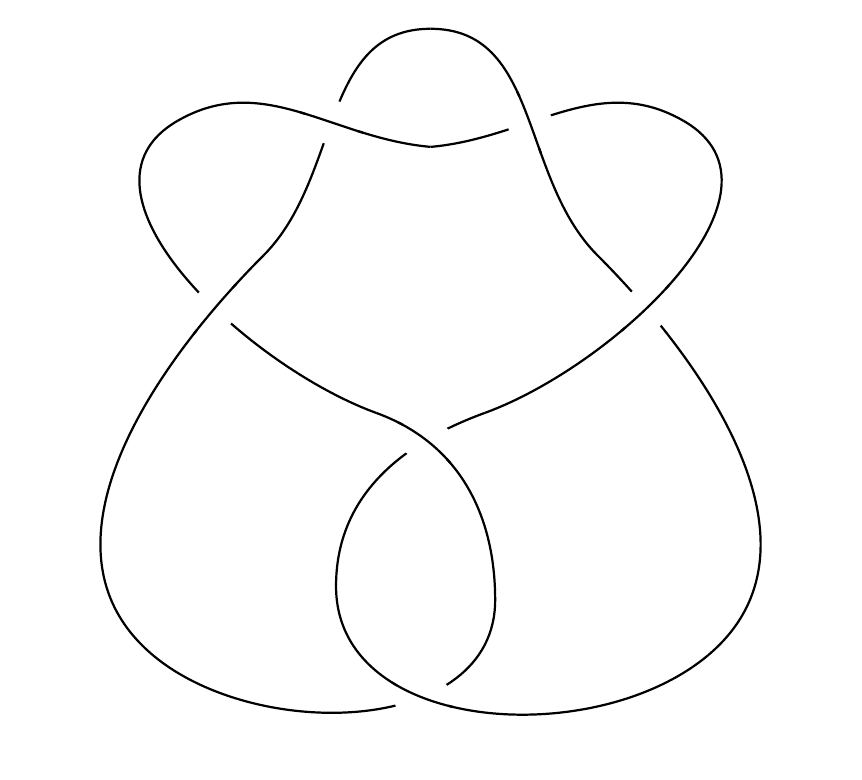
\begin{tikzpicture}[bgnd/.style={circle, fill=white, draw=white}]
    %\node[opacity=0.2] at (0,0) {\includegraphics[width=0.7\textwidth]{./rozdzialy/6_1-3d.png}};

    \coordinate (a0) at (0,0);
    \coordinate (a1) at (90:5);
    \coordinate (a2) at (45:3);
    \coordinate (a3) at (-40:4.6);
    \coordinate (a4) at (-120:2.4);
    \coordinate (a5) at (10:0.7);
    \coordinate (a6) at (50:5);
    \coordinate (a7) at (90:3.5);
    \coordinate (a8) at (180-50:5);
    \coordinate (a9) at (170:0.7);
    \coordinate (a10) at (-70:2.4);
    \coordinate (a11) at (220:4.6);
    \coordinate (a12) at (180-45:3);

    %\foreach \i in {0,...,12} \fill (a\i) circle (2pt);

    \begin{knot}[
      clip width=20, 
      flip crossing=1,
      flip crossing=3,
      flip crossing=6
      ]
      \strand[thick] (a1) to[out=0, in=90+45] (a2) to[out=-45, in=40] (a3);
      \strand[thick] (a3) to[out=220, in=-90] (a4) to[out=90, in=200] (a5);
      \strand[thick] (a5) to[out=20, in=-30] (a6);
      \strand[thick] (a6) to[out=150, in=5] (a7);
      \strand[thick] (a7) to[out=175, in=30] (a8);
      \strand[thick] (a8) to[out=210, in=160] (a9);
      \strand[thick] (a9) to[out=-20, in=90] (a10);
      \strand[thick] (a10) to[out=-90, in=-40] (a11);
      \strand[thick] (a11) to[out=140, in=180+45] (a12);
      \strand[thick] (a12) to[out=45, in=180] (a1);
    \end{knot}

    %\node at (80: 5) {$A$};
    %\node at (-40:4) {$B$};
    %\node at (45:5.5) {$C$};
    %\node at (135:5.5) {$D$};
    %\node at (-1.5,0.1) {$E$};
    %\node at (220:4) {$F$};
    %
    %\node[bgnd] at (70:4.7) {$1$};
    %\node[bgnd] at (25:3.9) {$2$};
    %\node[bgnd] at (-90:3) {$3$};
    %\node[bgnd] at (90:0.5) {$4$};
    %\node[bgnd] at (110:4.7) {$5$};
    %\node[bgnd] at (180-25:3.9) {$6$};

    %\draw[dashed] (70: 4) circle (0.4);
    %\draw[dashed] (28: 3.1) circle (0.4);
    %\draw[dashed] (-90:3.5) circle (0.4);
    %\draw[dashed] (-90:0.15) circle (0.4);
    %\draw[dashed] (180-28:3.1) circle (0.4);
    %\draw[dashed] (110:4) circle (0.4);
  \end{tikzpicture}
\end{center}

%\begin{center}
%  \begin{tikzpicture}
%    \begin{knot}[
%      consider self intersections,
%      flip crossing=2,
%      clip width=20,
%      ]
%      \strand[thick]
%      (90:3) to[out=180,in=-120,looseness=2]
%      (-30:3) to[out=60,in=120,looseness=2]
%      (210:3) to[out=-60,in=0,looseness=2] (90:3);
%    \end{knot}
%
%  %\fill (0,0) circle (2pt);
%  %\fill(90:2) circle (2pt);
%  %\fill(-30:2) circle (2pt);
%  %\fill(210:2) circle (2pt);
%  \end{tikzpicture}
%\end{center}
%
%\begin{center}
%  \begin{tikzpicture}
%    \begin{knot}[
%      consider self intersections,
%      flip crossing=2,
%      clip width=10,
%      ]
%      \strand[thick]
%      (120:2) to[out=180, in=180, looseness=2] (210:1) to[out=0, in=-140, looseness=1] (40:0.6) to[out=40, in=180, looseness=0.5] (40:1) to[out=5, in=-5, looseness=3] (-40:1) to[out=180, in=0, looseness=0.5] (150:1) to[out=180, in=180, looseness=2] (-120:2) to[out=0, in=0, looseness=1.3] (120:2);
%    \end{knot}
%%\fill (120:2) circle (2pt);
%%\fill (-120:2) circle (2pt);
%%\fill (-40:1) circle (2pt);
%%\fill (40:1) circle (2pt);
%%\fill (150:1) circle (2pt);
%%\fill (210:1) circle (2pt);
%%\fill[green] (40:0.6) circle (2pt);
%%\fill[red] (0,0) circle (2pt);
%  \end{tikzpicture}
%\end{center}
\newpage

%\section{Problem}

{\bfseries%
  Consider the ring $\Z[[F]$, where $[F]$ is the equivalence class of all finite abelian groups isomorphic to $F$. Describe the set $\Z[[F]]/\{[F_2]=[F_1]+[F_3]\}$, where relation $[F_2]=[F_1]+[F_3]$ means that there exists exact sequence:

  \begin{center}\begin{tikzcd}
    0\arrow[r] & F_1\arrow[r] & F_2\arrow[r] & F_3\arrow[r] & 0
  \end{tikzcd}\end{center}
}

Every finite abelian group is isomorphic to either a cyclic group or a finite product of cyclic groups. We will use this fact alongside the knowledge that every cyclic group is isomorphic with $\Z_n$ for some $n\in\N$.

We will start by showing that if $n=k\cdot l$ then $[\Z_n]=[\Z_k]+[\Z_l]$. Consider the sequence

\begin{center}\begin{tikzcd}
  0 \arrow[r] & \Z_k \arrow[r, "f"] & \Z_{n} \arrow[r, "g"] & \Z_l \arrow[r] & 0
\end{tikzcd}\end{center}

Define $f(1)=l\mod n$ and $g(1)=1\mod l$. We now need to check if $\ker g=\im f$. Take any $x\in\ker g$, then $x=l\cdot m\mod n$ for some $m\in\{0, 1, 2, ..., k-1\}$. Then for $m\mod l\in\Z_l$ we have $f(m\mod l)=ml\mod n$ and so $x\in\ker g\iff x\in \im f$. This shows that the sequence above is exact and $[\Z_n]=[\Z_k]+[\Z_l]$.

Furthermore, if $n=\prod_{i\leq m}k_i$, then
$$[\Z_n]=[\Z_{\prod_{i\leq m-1}k_i}]+[\Z_{k_m}]=...=\sum_{i\leq m}[\Z_{k_i}]$$
and if $n=p^k$ then by applying the above equation we have $[\Z_n]=k[\Z_p]$.

Next, we observe that for any $n,k\in\Z$ $[\Z_n\oplus \Z_k]=[\Z_n]+[\Z_k]$. This is because

\begin{center}\begin{tikzcd}
  0\arrow[r] & \Z_n \arrow[r, "f"] & \Z_n\oplus \Z_k \arrow[r, "g"] & \Z_k \arrow[r] & 0
\end{tikzcd}\end{center}

with $f(x)=x\oplus 0$ and $g(x\oplus y)=y$ is an exact sequence. For any $x\oplus y\in\ker g$ we must have $y=0$ while $x$ is unrestricted thus $x\oplus y\in \im f$.

From the latter statement, the following equality is immediately obtained:
\begin{align*}
  \Bigl[\bigoplus_{i\leq n}\Z_{k_i}\Bigr]=\Bigl[\bigl(\bigoplus_{i\leq n-1} \Z_{k_i}\bigr)\oplus \Z_{k_n}\Bigr]=\Bigl[\bigoplus_{i\leq n-1}\Z_{k_i}\Bigr]+[\Z_{k_n}]=...=\sum_{i\leq n}[\Z_{k_i}]
\end{align*}

If $F_n$ and $F_n'$ are two abelian groups of order $n$ and if $F_n=\bigoplus_{i\leq m}\Z_{k_i}$ then we have
$$[F_n]=\sum_{i\leq m} [\Z_{k_i}]$$
But because $n=|F_n|=|\oplus \Z_{k_i}|=\prod k_i$, then from the first two observations we obtain
$$[F_n']=\sum_{i\leq m} [\Z_{k_i}]$$
and so $[F_n]=[F_n']$. This allows us to replace every $\sum n_i[F_i]\in\Z[[F]$ with $\sum k_i[\Z_{p_i}]$ for prime $p_i$. Therefore,
$$\Z[[F]/\{[F_2]=[F_1]+[F_3]\}=\{\sum_{i\leq n} k_i[\Z_{p_i}]\;:\;p_i\text{ are prime}, n,k_i\in\N\}$$


%\section{Introduction}

\subsection{Order of an Ideal over PID ring}

PID -> every ideal is generated by one element, every module is an image of a free module, hence it can be expressed as $M\cong R/I_1\oplus...\oplus R/I_n$ for some ideals $I_i$. This allows as to define order of a module as $\ord(M)=\ord(I_1...I_n)$, which is the element that generates the ideal $I_1....I_n$. 

$\ord(M)$ can also be described using equivalence relation $M\sim M_1 + M_2\iff 0\to M_1\to M\to M_2\to 0$ is an exact sequence -> finitely generated abelian groups as $\Z$ modules and vector fields over $\mathfrak{K}$ as $\mathfrak{K}[x]$-modules.

\subsection{The Problem of non-PID rings}

Not every ring is a PID -> we must either find another invariant or make the ring in question a PID. E.g. for $\Z[x, x^{-1}]$ we can tensor it with some field, usually $\Q$ but we might want to try $F_p$ for some prime $p$.

Maybe some example for $\Z[x]$?

\subsection{Short Introduction to Knot Theory?}

Knot - a closed curve immersed in some $3$-dimensional space, or $S^1$ immersed in $S^3$

We will consider only tamed knots? That is knots that can be represented as a sum of a finite amount of straight lines?

Using Mayer-Vietoris sequence we can deduce that $H^1(S^3\setminus K)=\Z$ for any knot $K$. Hence, if we want to find interesting invariants, we must look further. 

Seifert surface of knot $K$ is an orientable surface whose boundary is $K$. We can use it to create an infinite cyclic covering of $S^3\setminus K$ by cutting copies $S^3\setminus K$ along this surface and gluing the $+$ side of Seifert surface of one copy to the $-$ side of the next copy.

$H^1(K^*)$ is more complicated than $H^1(S^3\setminus K)$ and things get interesting if we consider it as a $\Z[\Z]$ (or $\Z[x, x^{-1}]$-module. We can use the fact that $\Pi_1(K^*)^{ab}=H^1(K^*)$ and calculate this module to obtain something called Alexander ideal $I$: $H^1(K^*)\cong \Z[\Z]/I$. If $I$ is a principal ideal, e.g. in the case of trefoil knot of figure eight knot, its generator is called "Alexander polynomial". If this is not the case, we must consider $H^1(K^*; \Q)$ - kohomology module with coefficients in $\Q$, to obtain the Alexander polynomial. In the following paper we will consider what happens if we use $F_p$, a finite field, instead of $\Q$.


%\section{Calculating the Alexander Module}

Kinoshita-Tarasaki - does not look too promising

Conway Knot - to be examined


%\section{The case of oriented knot diagrams}

\subsection{Labeling homomorphism with orientation}

Every knot diagram can be endowed with orientation in two different ways. Given an oriented knot diagram there are two distinct types of crossings as seen in \cref{fig:4:two:types:crossings}. In such crossings segments $i$ and $o$ are easily distinguishable, allowing us to write two different elements to which labeling homomorphism $\phi$ will map segments that contribute to one crossing:
$$+:\phi(u,i,o)=au+bi+co$$
$$-:\phi(u,i,o)=\alpha u+\beta i+\gamma o.$$

\begin{figure}[h]\centering
  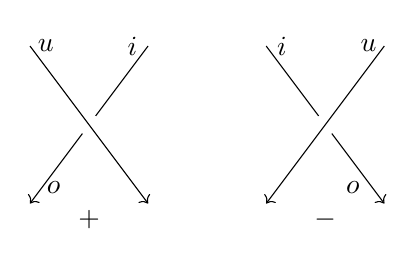
\begin{tikzpicture}
    \draw[<-] (0, -2)--(1.5, 0);
    \fill[white] (0.75, -1) circle (4pt);
    \draw[->] (0, 0)--(1.5, -2);

    \node at (0.75, -2.2) {$+$};
    \node at (0.2, 0) {$u$};
    \node at (1.3, 0) {$i$};
    \node at (0.3, -1.8) {$o$};

    \draw[->] (3, 0)--(4.5, -2);
    \fill[white] (3.75, -1) circle (4pt);
    \draw[<-] (3, -2)--(4.5, 0);
    
    \node at (3.75, -2.2) {$-$};
    \node at (3.2, 0) {$i$};
    \node at (4.3, 0) {$u$};
    \node at (4.1, -1.8) {$o$};
  \end{tikzpicture}
  \caption{\label{fig:4:two:types:crossings}Two types of crossings in oriented knot diagram.}
\end{figure}

Just as before, elements from $M^s$ that map to $0$ element in $M^x$ are responsible for coloring of the diagram being examined.

Those two definitions of homomorphism can be used to define two operators $M\times M\to M\times M$ which take segments that enter a crossing and return segments that leave said crossing. Looking from top to bottom of \cref{fig:4:two:types:crossings}, said operators are represented by matrices:
$$
A_+=\begin{pmatrix}
  -c^{-1}a & -c^{-1}b \\
  1 & 0
\end{pmatrix}
\begin{pmatrix}u\\i\end{pmatrix}
\quad\quad\quad
A_-=\begin{pmatrix}
  0 & 1 \\ 
  -\gamma^{-1}\beta & -\gamma^{-1}\alpha
\end{pmatrix}
\begin{pmatrix}i\\u\end{pmatrix}
$$


%\section{Problem}

Consider a field $\mathfrak{K}$ and the ring of polynomials with coefficients in $\mathfrak{K}$, $\mathfrak{K}[x]$. Obviously, the aforementioned ring is a principial ideal domain. We want to consider group $\Z[[M]]$, where $[M]$ is the equivalence class of all finitely generated torsion modules isomorphic to $M$ and relation $[M_2]=[M_1]+[M_3]$ defined by the existence of an exact sequence.

Any finitely generated module $M$ is isomorphic to a direct sum of cyclic modules:
$$M\cong p_1\mathfrak{K}[x]\oplus p_2\mathfrak{K}[x]\oplus...\oplus p_n\mathfrak{K}[x]$$

Moduły które mają ten sam wielomian w rozkładzie trafiają do tego samego domku.

{\color{green} If $p$, $q$ are two irreducible polynomials, then $(p)\oplus  (q)=\mathfrak{K}[x]$ (example: $x-1, x^2+1$).}


$$x^2+2x+1-(x-1)(x+3)$$


\section{Introduction}

\subsection{What does it mean to color a knot?}

What do we need?

- $R$ - commutative ring with identity

- $D$ - diagram of knot $K$ with $s$ segments and $x$ crossings

- $\phi:M^3\to M$ - function that dictates the rules of our coloring (and induces two operators $M^2\to M^2$)

In order for trivial coloring to work, $\phi(m,m,m)=0$ for all $m\in M$. This means that if we take $\phi(u, v, w)=au+bv+cw$ then $(a+b+c)\in\ann(M)$.

In the most general case, $R=\Z[s, t, t^{-1}]/\{s(s+t-1)\}$ and $\phi(u,v,w)=su+tv-w$.

Given those we can define $f:M^s\to M^x$, which assigns values from $M$ to segments of $D$ according to the rules set by $\phi$.

This yields an exact sequence
\begin{center}\begin{tikzcd}
  0\arrow[r] & \ker f\arrow[r, hookrightarrow] & M^s\arrow[r, "f"] & M^x \arrow[r, two heads] & \coker f \arrow[r] & 0 
\end{tikzcd}\end{center}

We know that $\ker f$ always contains colorings - especially the trivial one. We expect $\coker f$ to contain some information about non-trivial colorings admissible.

\subsection{Smith's normal form}

Function $f$ can be expressed as a $s\times x$ matrix with elements from $M$ - we can make it into "diagonal form" where non-zero elements lower are divisible by elements at the top. This gives us information about $\ker f$ and $\coker f$.

\begin{example}
  Take $K=4_1$ and $R=\Z$, which takes $t=1$ and $s=2$. At the beginning, $M=\Z$.

  \begin{center}
    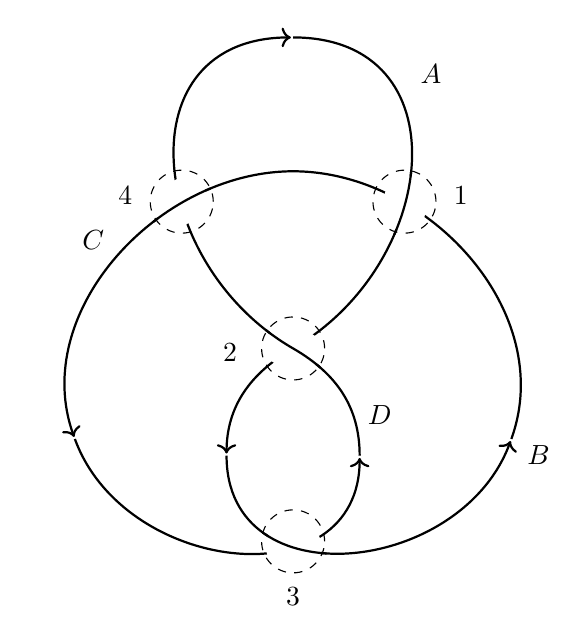
\begin{tikzpicture}
      %\node[opacity=0.2] at (0,0) {\includegraphics[width=0.5\textwidth]{./rozdzialy/4_1-3d.png}};
      \coordinate (a1) at (90: 3.5);
      \coordinate (a2) at (-30:3.2);
      \coordinate (a3) at (210: 3.2);
      \coordinate (a4) at (0,-0.45);
      \coordinate (a5) at (-65:2);
      \coordinate (a6) at (180+65: 2);
      \coordinate (a7) at (90: 1.8);

      %\foreach \i in {1, ..., 7} \fill (a\i) circle (2pt);
      \begin{knot}[
        %consider self intersections,
        flip crossing=2,
        clip width=20,
        ]
        \strand[thick, ->]
        (a1) to [out=0, in=30, looseness=1.4] 
        (a4) to [out=210, in=90, looseness=1] (a6);
        \strand[thick, ->]
        (a6) to [out=-90, in=250, looseness=1.3] (a2);
        \strand[thick, ->] (a2) to[out=70, in=0] (a7) to[out=180, in=110] (a3);
        \strand[thick, ->] (a3) to[out=290, in=-90, looseness=1.3] (a5);
        \strand[thick, ->] (a5) to[out=90, in=-30, looseness=1] (a4) to [out=150, in=180, looseness=1.4] (a1);
      \end{knot}
      \node at (60:3.5) {$A$};
      \node at (-30:3.6) {$B$};
      \node at (160:2.7) {$C$};
      \node at (1.1, -1.3) {$D$};

      \draw[dashed] (a4) circle (0.4);
      \node at (-0.8, -0.5) {$2$};

      \draw[dashed] (45:2) circle (0.4);
      \node at (35: 2.6) {$1$};

      \draw[dashed] (0, -2.9) circle (0.4);
      \node at (0, -3.6) {$3$};

      \draw[dashed] (135:2) circle (0.4);
      \node at (145:2.6) {$4$};
    \end{tikzpicture}
  \end{center}
  $$f=\begin{pmatrix} 
    2 & -1 & -1 & 0\\ 
    -1 & -1 & 0 & 2\\ 
    0 & 2 & -1 & -1 \\ 
    -1 & 0 & 2 & -1
    \end{pmatrix}$$
    in normal form:
  $$\begin{pmatrix}
    -1 & 0 & 0 & 0\\ 
    0 & 1 & 0 & 0\\
    0 & 0 & 5 & 0\\ 
    0 & 0 & 0 & 0
  \end{pmatrix}$$
  Now we know that $\ker f=\Z$ and $\coker f=\Z_5\oplus \Z$. Thus there is only a trivial coloring over $\Z$ but if we change $\Z$ to $\Z_5$ we get 
  $$\begin{pmatrix}
    -1 & 0 & 0 & 0\\ 
    0 & 1 & 0 & 0\\
    0 & 0 & 0 & 0\\ 
    0 & 0 & 0 & 0
  \end{pmatrix}$$
  and now $\ker f'=\Z_5\oplus \Z_5$ and $\coker = \Z_5\oplus\Z_5$. Thus there is a coloring using elements of $\Z_5$, for example:

  \begin{center}
    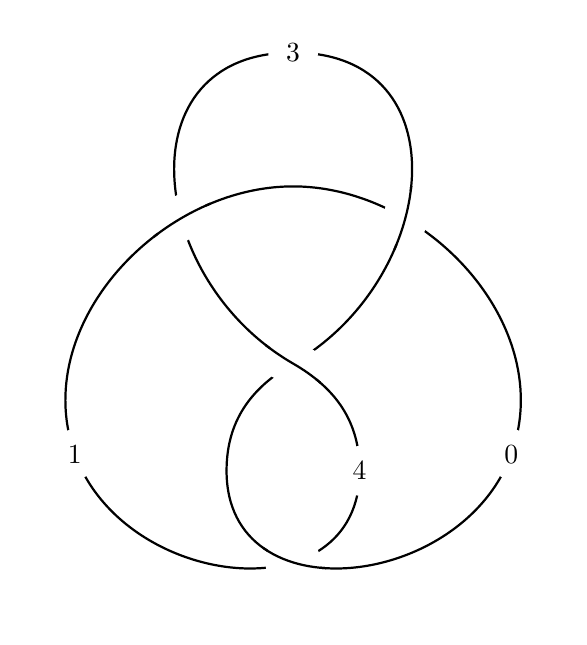
\begin{tikzpicture}[bgnd/.style={circle, fill=white, draw=white}]
      %\node[opacity=0.2] at (0,0) {\includegraphics[width=0.5\textwidth]{./rozdzialy/4_1-3d.png}};
      \coordinate (a1) at (90: 3.5);
      \coordinate (a2) at (-30:3.2);
      \coordinate (a3) at (210: 3.2);
      \coordinate (a4) at (0,-0.45);
      \coordinate (a5) at (-65:2);
      \coordinate (a6) at (180+65: 2);
      \coordinate (a7) at (90: 1.8);

      %\foreach \i in {1, ..., 7} \fill (a\i) circle (2pt);
      \begin{knot}[
        %consider self intersections,
        flip crossing=2,
        clip width=20,
        ]
        \strand[thick]
        (a1) to [out=0, in=30, looseness=1.4] 
        (a4) to [out=210, in=90, looseness=1] (a6);
        \strand[thick]
        (a6) to [out=-90, in=250, looseness=1.3] (a2);
        \strand[thick] (a2) to[out=70, in=0] (a7) to[out=180, in=110] (a3);
        \strand[thick] (a3) to[out=290, in=-90, looseness=1.3] (a5);
        \strand[thick] (a5) to[out=90, in=-30, looseness=1] (a4) to [out=150, in=180, looseness=1.4] (a1);
      \end{knot}

      \node[bgnd] at (a1) {$3$};
      \node[bgnd] at (a2) {$0$};
      \node[bgnd] at (a3) {$1$};
      \node[bgnd] at (a5) {$4$};
    \end{tikzpicture}
  \end{center}
  In a more general case, we would orient the diagram and use $\Z[\Z]=\Z[t, t^{-1}]$ as the ring:
  $$
  f=\begin{pmatrix}
    1-t & t & -1 & 0 \\ 
    t^{-1} & -1 & 0 & 1-t^{-1}\\ 
    0 & 1-t^{-1} & t^{-1} & -1\\ 
    -1 & 0 & 1-t & t
  \end{pmatrix}
  $$
  $$
  \begin{pmatrix}
    -1 & 0 & 0 & 0 \\
    0 & -1 & 0 & 0\\ 
    0 & 0 & t^2-3t+1 & 0\\ 
    0 & 0 & 0 & 0\\ 
  \end{pmatrix}
  $$
  and the Alexander polynomial of $4_1$ is equal to $t-3+t^{-1}$, which is the same up to multiplication by a unit to the last term of the Smith's normal form.
\end{example}














%{\color{blue}
%Let $D$ be a diagram of knot $K$ with $s$ segments and $x$ crossings.  We will take $R$ to be a commutative ring with identity and $M$ to be any $R$-module. Looking at each crossing locally, we see that exactly $3$ segments will meet and thus we need a function 
%$$\phi:M^3\to M$$ 
%which assigns value to a crossing based on the values inscribed on segments from which it is constructed.  
%
%We can now extend the function $\phi$ to work on the whole diagram $D$, which yields a new function 
%$$f:M^s\to M^x,$$
%that assigns values from $M$ to line segments from $D$. We say that $(x_1,...,x_s)\in M^s$ is a \emph{coloring of $D$} if 
%$$(x_1,...,x_s)\in\ker f,$$
%or in other words: $f(x_1,...,x_s)=0$.
%
%We want any trivial coloring to always be admissible and thus $a$, $b$, $c$ in the definition of $\phi$ must be from $\ann(M)$:
%$$0=\phi(m,m,m)=am+bm+cm=(a+b+c)m$$
%for all $m\in M$.
%
%On the other hand, function $\phi$ can be used to construct an operator $M^2\to M^2$ which takes segments entering a crossing and returns segments leaving it. In the case of a diagram with defined orientation, we can distinguish two types of crossings (look at \cref{fig:1:two:types:crossings}) and so $\phi$ will actually give rise to two different operators $A_{\pm}:M^2\to M^2$, whose composition is identity on $M^2$ (this is a direct result of Reidemeister moves).
%
%\begin{figure}[h]\centering
%  \begin{tikzpicture}
%    \draw[<-, thick] (0, -2)--(1.5, 0);
%    \fill[white] (0.75, -1) circle (6pt);
%    \draw[->, thick] (0, 0)--(1.5, -2);
%
%    \node at (0.75, -2.2) {$+$};
%    %\node at (0.2, 0) {$u$};
%    %\node at (1.3, 0) {$i$};
%    %\node at (0.3, -1.8) {$o$};
%
%    \draw[->, thick] (3, 0)--(4.5, -2);
%    \fill[white] (3.75, -1) circle (6pt);
%    \draw[<-, thick] (3, -2)--(4.5, 0);
%    
%    \node at (3.75, -2.2) {$-$};
%    %\node at (3.2, 0) {$i$};
%    %\node at (4.3, 0) {$u$};
%    %\node at (4.1, -1.8) {$o$};
%  \end{tikzpicture}
%  \caption{\label{fig:1:two:types:crossings}Two types of crossings in oriented knot diagram.}
%\end{figure}
%
%{\color{red}
%Having constructed two $2\times 2$ matrices, $A_+$ and $A_-$, from $\phi$ we can now represent $D$ as an element of braid group $W\in B_n$. This group has $(n-1)$ generators, $\sigma_1,...,\sigma_{n-1}$, to which we can assign matrices 
%$$\sigma_i=\left[
%\begin{array}{c|c|c}
%  Id_{i-1} & 0 & 0 \\ 
%  \hline 
%  0 & A_+  & 0 \\ 
%  \hline 
%  0 & 0 & Id_{n-i-1}
%\end{array}\right]
%$$
%Using these matrices we can now color this braid representation of $D$ to obtain a smaller matrix $B(W)$ than the one describing $f$ above. We will say that $(m_1,...,m_{s'})$ is a coloring of this braid diagram $W$ (which can have $s'\neq s$ segments) if $(m_1,...,m_{s'})\in\ker B(W)$.
%}
%}
%


\subsection{Misc}

$K=6_1$

\begin{center}
  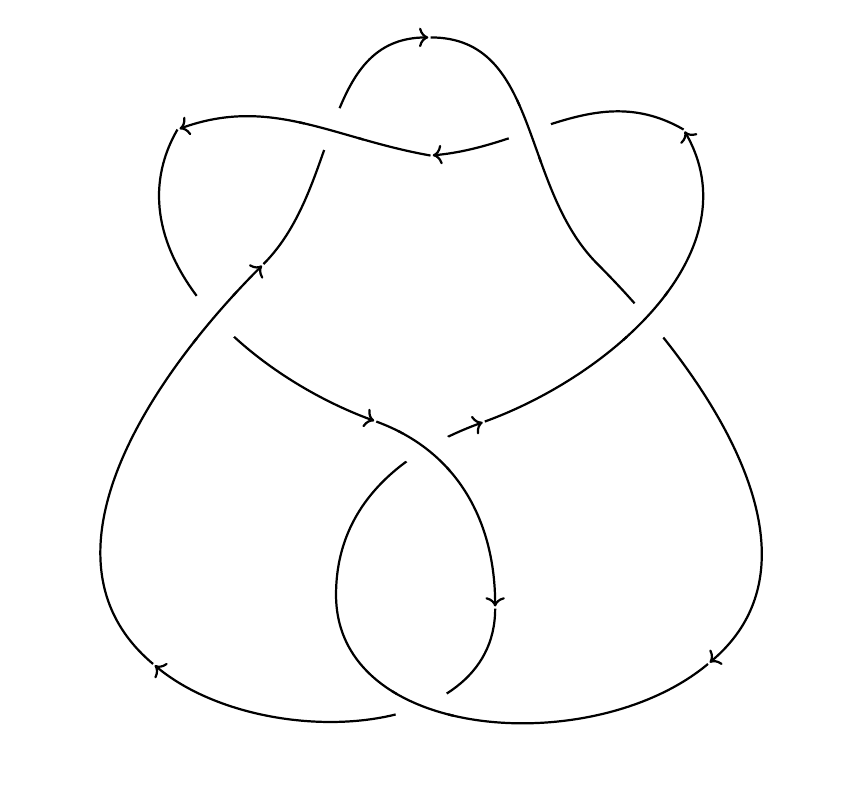
\begin{tikzpicture}[bgnd/.style={circle, fill=white, draw=white}]
    %\node[opacity=0.2] at (0,0) {\includegraphics[width=0.7\textwidth]{./rozdzialy/6_1-3d.png}};

    \coordinate (a0) at (0,0);
    \coordinate (a1) at (90:5);
    \coordinate (a2) at (45:3);
    \coordinate (a3) at (-40:4.6);
    \coordinate (a4) at (-120:2.4);
    \coordinate (a5) at (10:0.7);
    \coordinate (a6) at (50:5);
    \coordinate (a7) at (90:3.5);
    \coordinate (a8) at (180-50:5);
    \coordinate (a9) at (170:0.7);
    \coordinate (a10) at (-70:2.4);
    \coordinate (a11) at (220:4.6);
    \coordinate (a12) at (180-45:3);

    %\foreach \i in {0,...,12} \fill (a\i) circle (2pt);

    \begin{knot}[
      clip width=20, 
      flip crossing=1,
      flip crossing=3,
      flip crossing=6
      ]
      \strand[thick, ->] (a1) to[out=0, in=90+45] (a2) to[out=-45, in=40] (a3);
      \strand[thick, ->] (a3) to[out=220, in=-90] (a4) to[out=90, in=200] (a5);
      \strand[thick, ->] (a5) to[out=20, in=-60] (a6);
      \strand[thick, ->] (a6) to[out=150, in=5] (a7);
      \strand[thick, ->] (a7) to[out=170, in=20] (a8);
      \strand[thick, ->] (a8) to[out=240, in=160] (a9);
      \strand[thick, ->] (a9) to[out=-20, in=90] (a10);
      \strand[thick, ->] (a10) to[out=-90, in=-40] (a11);
      \strand[thick, ->] (a11) to[out=140, in=180+45] (a12);
      \strand[thick, ->] (a12) to[out=45, in=180] (a1);
    \end{knot}

    %\node at (80: 5) {$A$};
    %\node at (-40:4) {$B$};
    %\node at (45:5.5) {$C$};
    %\node at (135:5.5) {$D$};
    %\node at (-1.5,0.1) {$E$};
    %\node at (220:4) {$F$};
    %
    %\node[bgnd] at (70:4.7) {$1$};
    %\node[bgnd] at (25:3.9) {$2$};
    %\node[bgnd] at (-90:3) {$3$};
    %\node[bgnd] at (90:0.5) {$4$};
    %\node[bgnd] at (110:4.7) {$5$};
    %\node[bgnd] at (180-25:3.9) {$6$};

    %\draw[dashed] (70: 4) circle (0.4);
    %\draw[dashed] (28: 3.1) circle (0.4);
    %\draw[dashed] (-90:3.5) circle (0.4);
    %\draw[dashed] (-90:0.15) circle (0.4);
    %\draw[dashed] (180-28:3.1) circle (0.4);
    %\draw[dashed] (110:4) circle (0.4);
  \end{tikzpicture}
\end{center}
Tutaj mamy
$$f=\begin{pmatrix}
  -1 & 0 & 0 & 0 & 0 & 0 \\ 
  0 & -1 & 0 & 0 & 0 & 0 \\ 
  0 & 0 & t & 0 & 0 & 0 \\ 
  0 & 0 & 0 & t & 0 & 0 \\ 
  0 & 0 & 0 & 0 & -2t^{-2}+5t^{-1}-2 & 0 \\ 
  0 & 0 & 0 & 0 & 0 & 0 
\end{pmatrix}$$

$K=9_{46}$
\newpage 

\begin{center}
  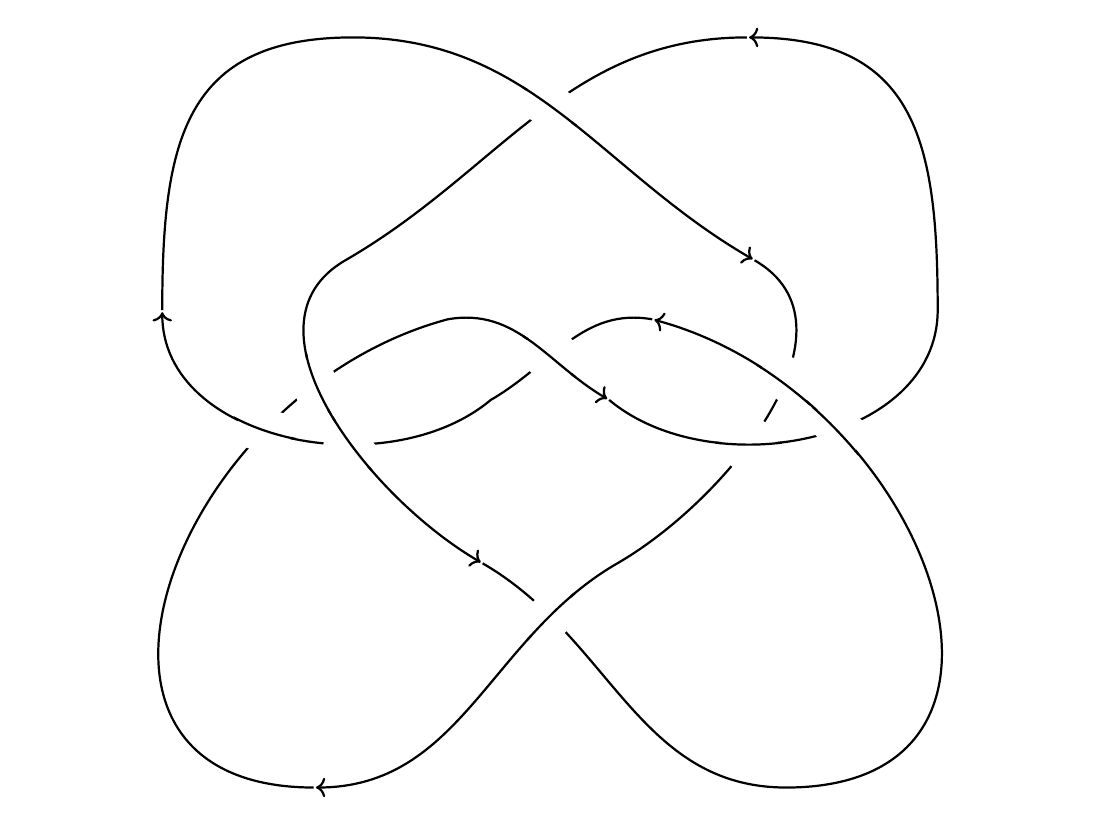
\begin{tikzpicture}[bgnd/.style={circle, fill=white, draw=white}]
    %\node[opacity=0.2] at (0,0) {\includegraphics[width=0.7\textwidth]{./rozdzialy/6_1-3d.png}};

    \coordinate (a0) at (0,0);
    \coordinate (a1) at (60:5);
    \coordinate (a2) at (150:3);
    \coordinate (a3) at (-110:2.5);
    \coordinate (a4) at (-60:6);
    \coordinate (a5) at (30:1.5);
    \coordinate (a6) at (200:0.8);
    \coordinate (a7) at (170:5);
    \coordinate (a8) at (120:5);
    \coordinate (a9) at (30:3);
    \coordinate (a10) at (-70:2.5);
    \coordinate (a11) at (180+60:6);
    \coordinate (a12) at (150:1.5);
    \coordinate (a13) at (-20:0.8);
    \coordinate (a14) at (10:5);

    %\foreach \i in {0,...,14} \fill (a\i) circle (2pt);

    \begin{knot}[
      clip width=20, 
      consider self intersections,
      ignore endpoint intersections=false,
      %draft mode=crossings,
      flip crossing=1,
      flip crossing=4,
      flip crossing=7, 
      flip crossing=9
      ]
      \strand[thick, ->] 
        (a1) to [out=180, in=30]
        (a2) to [out=210, in=150]
        (a3);
      \strand[thick, ->]
        (a3) to [out=-30, in=180] 
        (a4) to [out=0, in=-15, looseness=1.5] 
        (a5);
      \strand[thick, ->]
        (a5) to [out=170, in=30] 
        (a6) to [out=220, in=-90] 
        (a7);
      \strand[thick, ->]
        (a7) to [out=90, in=180, looseness=1.3] 
        (a8) to [out=0, in=150] 
        (a9);
      \strand[thick, ->]
        (a9) to [out=-30, in=30]
        (a10) to [out=210, in=0] 
        (a11);
      \strand[thick, ->]
        (a11) to [out=180, in=180+15, looseness=1.5] 
        (a12) to [out=10, in=150]
        (a13);
      \strand[thick, ->]
        (a13) to [out=-40, in=-90]
        (a14) to [out=90, in=0, looseness=1.3]
        (a1);
      \fill[yellow] (-10:3.7) circle (6pt);
    \end{knot}
  \end{tikzpicture}
\end{center}

$$f=\begin{pmatrix}
  1 & 0 & 0 & 0 & 0 & 0 & 0 & 0 & 0 \\ 
  0 & t^{-1} & 0 & 0 & 0 & 0 & 0 & 0 & 0 \\ 
  0 & 0 & t^{-1} & 0 & 0 & 0 & 0 & 0 & 0\\ 
  0 & 0 & 0 & t  & 0 & 0 & 0 & 0 & 0 \\ 
  0 & 0 & 0 & 0 & t  & 0 & 0 & 0 & 0 \\ 
  0 & 0 & 0 & 0 & 0 & t  & 0 & 0 & 0\\ 
  0 & 0 & 0 & 0 & 0 & 0 & 2t-t^2 & 0 & 0 \\ 
  0 & 0 & 0 & 0 & 0 & 0 & 0 & t^{-2}-2t^{-1} & 0\\ 
  0 & 0 & 0 & 0 & 0 & 0 & 0 & 0 & 0
\end{pmatrix}$$


\bibliographystyle{plain}
\bibliography{literatura}
 
\end{document}
